\chapter{A kiberbiztonsági analízis metodológiája}

A diplomamunkám legfontosabb része a metodológia előállítása volt. A metodológia az ami biztosítja azoknak a céloknak az elérését, hogy az analízis (i) teljes körű legyen, (ii) megismételhető legyen és (iii) már létező információkra építsen, azon túl, hogy az eredménye és használata minél átláthatóbb legyen a stakeholderek és az elemző mérnök számára is.

Ez a metodológia kapcsolja össze az autóiparra jellemző rendszermodelleket a fenyegetésmodellekkel. Ennek segítségére és támogatására készült el a kapcsolódó modellező eszköz és ennek az eredménye az egyik legfontosabb előállított értéke a kiberbiztonsági mérnök feladatkörnek.

Az említett fejezetben a példáimat egy tetszőleges személygépjármű kormányrendszerének az aktuációs (actuation: mozgásba hoz működtet) funkcionalitására készítettem el. 

Az \textit{Áttekintés} fejezet tartalmaz egy magas szintű végigvezetést a bemenetektől a kimenetig és a közte megtett lépésekről.

A \textit{Termékleírás és fenyegetésmodell származtatása} mutatja be a kiindulómodell elkészítésének lépéseit valamint, hogy abból, hogyan állítjuk elő a fenyegetés modellt.

A \textit{Fenyegetésmodellezés} fejezetben láthatóak a további lépések a fenyegetésmodell specifikálására, valamint be mutatja a fenyegetésmodellből előállított támadási fák konstrukcióját és annak szerkesztésének lépéseit.

A \textit{Dokumentumok generálása és manuális analízis} fejezetben pedig találhatóak a szabvány által előírt output előállítása és az elemző eszköz használatát követő folyamatok.

\section{Áttekintés}

A metodológiám fő feladata a \textit{Háttérismeretek} fejezetben található \textit{Követelmények a fenyegetéselemzésre és kockázatértékelésre} részben leírtakat követve kialakítsam azt a lépéssorozatot amelyet az általam fejlesztett eszköz támogatásával végre lehet hajtani és el lehet jutni egy általános autóipari modellből a kockázatelemzés eredményéig.

A lépésekről egy áttekintés a \ref{fig:04_OVERVIEW} ábrán látható. Itt egyrészről a fehér hátterű négyzetekben az ISO 21434 által definiált lépések láthatóak amelyek bővebb leírása a \textit{Háttérismeretek} részben található, lila hátterű négyzetekben pedig az ebben a fejezetben bemutatott lépések láthatóak. Így látható egy egyszerűbb áttekintés a két módszertan közti fedettségről.

\begin{figure}[!ht]
	\centering
	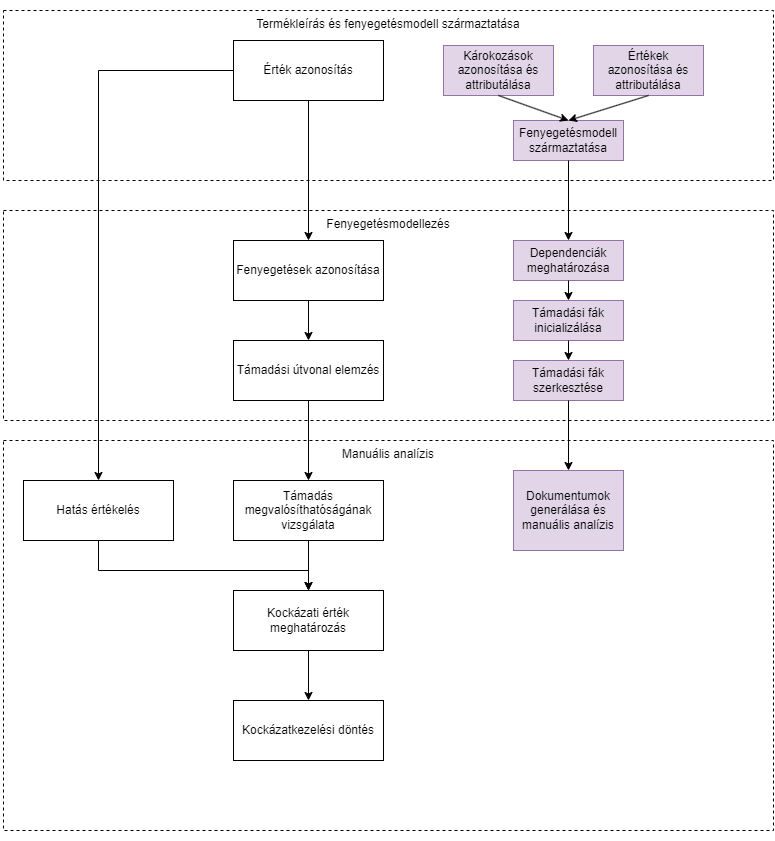
\includegraphics[width=130mm, keepaspectratio]{figures/04_overview.png}
	\caption{Metodológia áttekintése}
	\label{fig:04_OVERVIEW}
\end{figure}

\section{Termékleírás és fenyegetésmodell származtatása}

Ez a fejezet mutatja be az első lépéseit a kockázatelemzési folyamatnak. Itt lesz szükségünk a kiinduláskor rendelkezésünkre álló termékleírást (ami a rendszermodell egy részhalmaza) bővíteni kiberbiztonsági attribútumokkal majd abból származtatni egy olyan új modellt ami a kiberbiztonsági elemzésre alkalmas lesz.

Ehhez a rendszermodellünkben két diagram típusra lesz szükség. Az egyik a viselkedési diagramok közé sorolható használati eset (use case) diagram, a másik pedig egy strukturális kategóriába sorolható komponens diagram.\\

A használati eset diagramot a továbbiakban nevezzük \textit{kihasználási eset (abuse case)} diagramnak. Ez annyiban módosítja az eredeti diagram használatát, hogy amíg a szintaktikailag és szemantikailag ugyanaz, tartalmilag nem a felhasználó és rendszer közti kapcsolatokat keressük, hanem a támadó lehetséges motivációját és amit ténylegesen meg is tud tenni a rendszerrel. 

A kihasználási esetek azonosításában már tudjuk használni a CIA triád alkalmazását is. A bemutatott eljárásban, veszünk egy funkcionalitást amit a vizsgált termék ellát és azt finomítjuk tovább az egyes kiberbiztonsági tulajdonságoknak a sérülése szerint. Egy példa a \ref{fig:04_abuse_case} ábrán látható.

\begin{figure}[!ht]
	\centering
	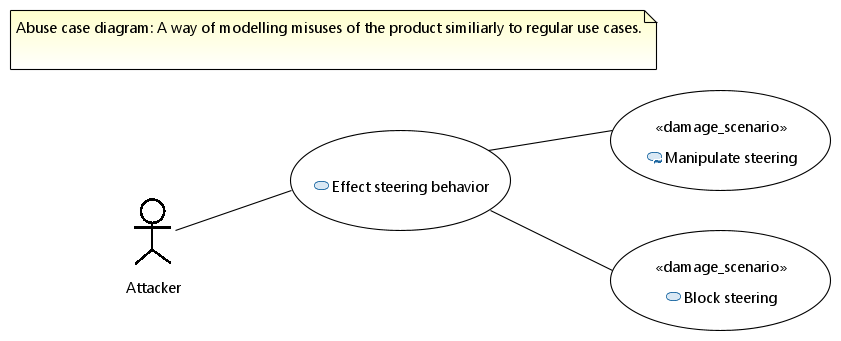
\includegraphics[width=130mm, keepaspectratio]{figures/04_abuse_case.png}
	\caption{Példa kihasználási eset diagramra}
	\label{fig:04_abuse_case}
\end{figure}

A példán jól látható, hogy amíg az "Effect steering behavior" tekinthető is lenne elvárt működésnek egy kormányrendszer esetén, addig amikor ez egy támadó lehetséges céljai közé tartozik akkor már nevezhető ez egy kihasználási esetnek. Ezt tudjuk tovább finomítani aszerint, hogy mely kiberbiztonsági tulajdonság sérülhet. Az eljárásban használt tulajdonságok a bizalmasság, sértetlenség és elérhetőség, ezek bővebben a \textit{Háttérismeretek} fejezetben kerültek bemutatásra. A "Manipulate steering" esetében az aktuáció sértetlenségi attribútuma sérül, a "Block steering" esetén pedig az elérhetősége. Bizalmassági tulajdonsága nincsen az aktuációnak, hiszen ennek a működtetése kívülről nem igényel semmilyen személyes adatot, szellemi terméket vagy kriptográfiai információt.

Az ISO 21434 szerint\\

A komponens diagram lesz, az ISO 21434 megnevezése szerint, a termékleírás (item definition). Ennek célja, hogy 

\subsection{Károkozások azonosítása és attributálása}



\subsection{Értékek azonosítása és attributálása}

\subsection{Fenyegetésmodell származtatása}

\section{Fenyegetésmodellezés}

\subsection{Dependenciák meghatározása}

\subsection{Támadási fák inicializálása}

\subsection{Támadási fák szerkesztése}

\section{Dokumentumok generálása és manuális analízis}